%%%%%%%%%%%%%%%%%%%%%%%%%%%%%%%%%%%%%%%%%%%%%%%%%%%%%%%%%%%%%%%%%%%%%%%
%%%                           SECTION V
%%%%%%%%%%%%%%%%%%%%%%%%%%%%%%%%%%%%%%%%%%%%%%%%%%%%%%%%%%%%%%%%%%%%%%

\chapter{\uppercase {Mouse embryonic stem cell-derived neuron high-throughput drug screen assay for Angelman syndrome}}

\subsubsection*{Abstract}

High-throughput drug discovery efforts for neurological disorders often rely on the use of mouse primary neuronal cultures; however, establishing primary cultures from the rodent brain is labor intensive, expensive and provides only a limited supply of cells. Mouse embryonic stem cell-derived neurons are an ideal alternative to primary cultures, because large quantities of cells are easily generated and readily differentiated into neurons in vitro, providing an almost unlimited source of cells for high-throughput screening (HTS) assays. Here, we developed and validated an ES cell-based HTS method to identify new therapies for Angelman syndrome (AS), a severe neurodevelopmental disorder that is caused by loss of the maternally inherited \textit{UBE3A} allele. In neurons, \textit{UBE3A} is imprinted with maternal-specific expression, thus leaving the paternal allele transcriptionally inactive but genetically intact. As such, approaches to reactivate expression of the paternal allele are seen as a viable therapeutic option for AS. ES cells with a paternally inherited \textit{Ube3a$^{YFP}$} reporter allele were generated to perform proof-of-concept HTS. Imprinted paternal \textit{Ube3a$^{YFP}$} is reactivated after treatment with Topotecan, a topoisomerase inhibitor known to reactivate the silenced paternal allele. These initial results demonstrate the utility of ES-N to perform HTS to identify novel therapeutics for neurological disorders.

\section{Introduction}

High-throughput screening (HTS) of drug libraries, small molecule compounds, and biologicals is a powerful approach to identify new therapies for a wide rand of diseases \cite{Aubi2015,Holbeck2004,Macarron2011,Seto2015,Stewart2015a,Stone2015,White1998,Zhang2007}. While most high-throughput drug discovery assays are relatively straightforward, those aimed at identifying new therapies for diseases of the central nervous system (CNS) are difficult because of the challenges associated with using neuronal cell-lines. Indeed there are numerous sources of immortalized neuronal cell-lines (e.g., P19, SH-SY5Y neuroblastoma cells, NT2, PC12 cells, etc.), but genetically modified mouse primary neurons are the most appropriate cell-line for performing high-throughput drug discovery screens for monogenic disorders \cite{Bernstock2016,Berry2015,Eglen2008,Gordon2015,Kaltenbach2010,Mazzio2015,Pouton2007,Schulte2011,Stewart2015b}. Methods currently used to establish mouse primary neurons involve immature neurons isolated from either prenatal (e.g., E15-E18) or early postnatal (e.g., P1-P2) brains. As such, scheduling experiments is entirely dependent on the breeding schedules and availability of mice.

The number of neurons obtained from the mouse brain is also rather limited; for example, current studies estimate that approximately 600,000 neurons per hippocampi and 800,000 neurons per cortice can be cultured per mouse brain \cite{Beaudoin2012}. Primary neuronal cultures are typically grown at 20,000 cells/well \cite{Huang2012}, approximately $7.68$ $\times$ $10^6$ cells would be needed for one 384-well plate. Mouse neural stem cells can be expanded \textit{in vitro}, but they can only be maintained in an undifferentiated state for a finite period of time, and they yield low percentages of neurons after differentiation. Another challenge is that most HTS facilities do not accommodate experiments involving primary cell cultures because of the risks associated with contaminating other cell-lines (personal communication Clifford Stephen). Altogether, high-throughput drug discovery efforts for neurological disorders are met with numerous technical challenges that have likely impeded drug discovery efforts.

Mouse embryonic stem (ES) cell-derived neurons are an ideal alternative to primary neuronal cultures. Mouse ES cells rapidly divide \textit{in vitro} and can be maintained in an undifferentiated state almost indefinitely. They are amendable to targeted genetic modifications or can easily be generated from existing transgenic models \cite{Gonzalez2014,Vasileva2015,Wang2012,Zhu2014}. They are commonly used in HTS assays and accepted by most all HTS facilities \cite{Desbordes2008}. Importantly, ES cells can be reliably and efficiently differentiated into neuronal cell populations that exhibit gene expression patterns, epigentic marks, and electrophysiological properties similar to mouse primary neurons \cite{Benninger2003,Garcia2012,Kim2002,Weick2011,Young2014}. Their use in high-throughput drug discovery assays, however, has been underutilized \cite{Breier2008,Koike-Yusa2014,Sadek2008,Tumarkin2011,Yoshikawa2006}.

Angelman syndrome (AS) is a debilitating neurodevelopmental disorder characterized by severe intellectual disability, absent speech, ataxia, seizures, frequent smiling and inappropriate laughter \cite{Kishino1997,Matsuura1997,Williams2006}. The genetic or epigenetic mutations causing AS are associated with loss of maternal - but not paternal - expression of the ubiquitin ligase E3A protein gene (\textit{UBE3A}). The non-Mendelian inheritance pattern of AS is due to genomic imprinting of \textit{UBE3A} \cite{Kishino1997,Matsuura1997}. In almost all cell-types, \textit{UBE3A} is expressed from both parental alleles; however, in the brain, \textit{UBE3A} is perferentially expressed from the maternal allele \cite{Yamasaki2003}. Expression of the paternal \textit{UBE3A} allele is inhibited by the antisense expression of a long polycistronic transcription unit (PTU) that is comprised of \textit{SNURF-SNRPN}, clusters of C/D box small nucleolar RNAs (\textit{SNORD64, SNORD109, SNORD116,} and \textit{SNORD115}), and the \textit{UBE3A} antisense transcript (\textit{UBE3A-AS}) \cite{Meng2012,Meng2013}). Studies in mice show that \textit{Ube3a} is imprinted in neurons, including ES cell-derived neurons, and biallelically expressed in other cell-types of the brain \cite{Landers2004,Rougeulle1998,Runte2004,Yamasaki2003}, which is consistent with the neuron-specific expression of \textit{UBE3A-AS}.

Currently, there are few treatment options for Angelman syndrome patients. Available treatments for those with Angelman syndrome focus on behavioral and physical therapies to minimize symptoms, along with drug therapies to control seizures and sleep disruption. Since the inactive paternal \textit{UBE3A} allele is genetically intact but epigenetically silent, approaches to reactivate expression of the paternal \textit{UBE3A} allele are therefore seen as viable therapeutic options to treat AS. In fact, recent studies in mice have shown that pharmacological, genetic, and epigenetic methods are all capable of reactivating expression of paternal \textit{Ube3a} expression in primary neurons and the adult mouse \cite{Bailus2016,Huang2012,Meng2013,Meng2015}. Importantly, there appears to be some degree of improvement of symptoms after reactivation \cite{Elgersma2007,Meng2015,Shi2015,Silva-Santos2015}.

In this study, we established and validated a fluorescence based HTS assay in ES cell-derived neurons (ES-N) with an \textit{Ube3a$^{YFP}$} reporter allele. We demonstrate the utility of this approach for performing large-scale, high-throughput drug discovery assays to identify novel therapies to treat Angelman syndrome.

\section{Materials and Methods}

\subsection{Animals}

Animals housed under the standard conditions, pathogen-free mouse facility. All procedures performed according to NIH guidelines and approved by the Texas A\&M University Institutional Animal Care and Use Committee (IACUC). The laboratory of Dr. Arthur Beaudet generated and provided \textit{Ube3a$^{YFP}$} mouse model \cite{Dindot2008}. All mice maintained on C57BL/6J background (The Jackson Laboratories, Bar Harbor, ME).

\subsection{Generation of \textit{Ube3a$^{+/YFP}$} embryonic stem cells}

Mouse \textit{Ube3a$^{+/YFP}$} ES cells were established following standard methods \cite{Behringer2014,Conner2001,Czechanski2014,Luo2011,Nagy2003}. Briefly, \textit{Ube3a$^{YFP/YFP}$} males were mated to three to four week old C57BL/6J superovulated female mice. Embryos (E2.5) collected from oviducts were cultured overnight in one well of a 4-well plate (Thermo Scientific, Waltham, MA) in KSOM Evolve (IVFonline, Guelph, Canada) containing 1 mg/ml bovine serum albumin (Sigma-Aldrich, St. Louis, MO). The following day, individual embryos were transferred and cultured for four days in 30 $\mu$l microdrops of KORS+2i medium covered by mineral oil (37$^{\circ}$C, 5\% CO$_2$) \cite{Gertsenstein2010,Luo2011}. After 96 h in KOSR-2i medium, outgrowths were trypsinized using 0.25\% Trypsin-EDTA (Life Technologies, Carlsbad, CA) into single-cell suspensions and plated individually in 96-well, flat bottom, tissue culture treated plate (Corning Inc., Corning, NY) containing a mitomycin-C inactivated SNL 76/7 feeder cells monolayer \cite{McMahon1990,Okita2007,Takahashi2007,Takahashi2009} (Applied StemCell, Milpitas, CA) at 50,000 cells/cm$^{2}$ and KOSR-2i preconditioned ($>$2 h) medium. Cells were incubated (37$^{\circ}$C, 5\% CO$_2$) for four days with daily changes of medium. To establish ES cell-lines, undifferentiated colonies were gradually expanded and genotyped using Jackson Laboratory genotyping primers for \textit{Ube3a$^{YFP}$}: 5' TCAATGATAGGGAGATAAAACA 3', 5' GAAAACACTAACATGGAGCTC 3', and 5' CTTGTGTAGCGCCAAGTGC 3'. Of the six lines tested for ES cell growth, lines \#2 and \#10 were selected for further large-scale expansion resulting in 43 vials at $3.5 \times 10^6$ cells/vial each. The following studies were conducted using line \#10.

\subsection{Neuronal Differentiation}

Retinoic acid based-induction methods \cite{Bibel2007,Kiris2011,Wu2012} with slight modifications for high-throughput screening purposes directed differentiation of \textit{Ube3a$^{+/YFP}$} ES cells into neuronal cultures as described in \textbf{Chapter 4}. For the dissociation step, ES cell-derived neurons cellular aggregates were transported to HTS facility ($\sim$37$^{\circ}$C, $\sim$2 h) or dissociated immediately in the lab. Either way, cells were dissociated with 0.5\% Trypsin-EDTA and plated in N2 media, \textbf{Table \ref{table:4-1}} on 384-well poly-d-lysine coated optical bottom plates (Thermo Scientific) at 24,000 cells/well using a microplate washer (Tecan Group Ltd, M\"{a}nnedorf, Switzerland) for HTS or 18 mm round coverslips (VWR, Radnor, PA) coated with poly-l-ornithine (Sigma-Aldrich) and laminin (Life Technologies) at $4 \times 10^5$ cells/well for imprint analysis. Stocks of 0.5 mg/ml poly-l-ornithine in 150 mM boric acid were diluted 1:5 in water to coat overnight at 4$^{\circ}$C. After coverslips were rinsed three times with cell culture grade water, laminin (10 $\mu$g/$\mu$l) was added to the coverslips and incubated at 4$^{\circ}$C overnight. After 48 h, medium was changed to Complete media, \textbf{Table \ref{table:4-1}}. Every three days Complete media was changed. Eight days post dissociation (DPD), compounds were added and maintained for 72 h. Topotecan hydrochloride (Sigma-Aldrich), was dissolved in water (10 mM stock) and then diluted to 3 $\mu$M into DMSO (Sigma-Aldrich) for HTS, while 10 $\mu$M stock in water was used for imprint analysis. Topotecan hydrochloride was added to plates at 300 nM final concentration along with vehicle (DMSO or water) using microplate washer for HTS or by-hand for imprint analysis as positive and negative controls, respectively.

\subsection{Immunocytochemistry}

Immunocytochemistry and staining were performed as described previously \cite{Watase2002}. Briefly, cells were fixed with 4\% paraformaldehyde (Sigma-Aldrich) for HTS or 4\% paraformaldehyde/ 4\% sucrose (Sigma-Aldrich) for imprint analysis (10 min, RT). For high-throughput drug screening, cultures were blocked in 5\% goat serum (Sigma-Aldrich) and 0.3\% Triton X-100 (Sigma-Aldrich) for 15 min at 37$^{\circ}$C, while imprint analysis blocked for 1 h at room temperature. Primary antibody was diluted in antibody buffer containing 5\% goat serum and 0.3\% Triton X-100 and incubated for 1 h at room temperature or for 30 min at 37$^{\circ}$C for the high-throughput screen. Cells were washed three times before secondary antibody incubation with 0.1\% Tween20 (Sigma-Aldrich) for 10 to 15 min at room temperature. Primary antibodies used here are as follows: anti-GFP (Novus Biologicals, Inc., Littleton, CO), anti-NeuN (EMD Millipore) and anti-$\beta$III Tubulin (Sigma-Aldrich). Secondary antibodies used was Alexa Fluor 488, goat anti-rabbit, and Cy3 goat anti-mouse (Jackson Immuno Research Labs, West Grove, PA). Secondary antibodies were incubated in 5\% goat serum and 0.3\% Triton X-100 for 1 h at room temperature for imprint analysis or for 30 min at 37$^{\circ}$C for high-throughput screening. TO-PRO-3 stain (Life Technologies) at 1:1000 dilution was used for nuclei staining. Images were captured using IN Cell 6000 (GE, Schenectady, NY), and confocal images were captured using Zeiss 510 META Confocal Microscope (Zeiss, Oberkochen, Germany). 
\subsection{Image analysis}
\subsubsection*{Imprint analysis}

For imprint analysis, FIJI (FIJI is just Image J, open source) was used in image preparation and to measure gray scale values of individual neurons \cite{Schindelin2012,Schneider2012}. Positive \( \beta \)III tubulin staining identified neurons. The Ube3a$^{YFP}$ fluorescence, GFP staining, of each neuron was expressed as YFP intensities overlapping neuronal TO-PRO-3 staining. Two-tailed unpaired Student's t-test was used to determine statistical significance when comparing two groups. To determine statistical significance for the time course, Holm-Bonferroni method was used to control the family-wise error rate for multiple comparisons.

\subsubsection*{HTS analysis}

Image analysis for high-throughput screening was performed using IN Cell Developer Toolbox 9.3.1. The TO-PRO-3, nuclei marker, and the NeuN, mature neuron marker, were used to generate a neuron specific overlapping mask, (\textbf{NeuN-Overlap}), which was used to measure median YFP intensity in each target. Several R scripts (\textbf{Appendix D}) were developed to analyze data rapidly for plate effects, within plate effects, and assay statistics. To determine statistical significance between plates, one-sided unpaired Student's t-test was used (multiple comparisons, Holm-Bonferroni method), along with the strictly standardized mean difference (SSMD). To determine statistical significance within plate, two-tailed unpaired Student's t-test was used.

\subsection{Charts}

Charts designed in R (version 3.2.2 \cite{Rcite2016}) programming using the tikzDevice package. \textbf{Appendix D} shows sample scripts.

\section{Results}

\subsection{Topotecan induces reactivation of silenced paternal \textit{Ube3a} allele in ES cell-derived neurons}

It has been established that ES-N can recapitulate the paternal imprint in ES cells \cite{Kohama2012,Meng2012}; however, a time course for this paternal imprint has not been established to the best of our knowledge. Here, we verified paternal imprint of \textit{Ube3a} via a 13 day time course to determine the days post dissociation (DPD) needed for the imprint to be established in this cell-line. \textbf{Figure \ref{Figure 5-1: }A} shows that after 6 days in culture paternal Ube3a$^{YFP}$ expression significantly decreased (\textbf{Table \ref{table:5-1}}, Holm-Bonferroni) and continues to maintain a low level of expression. By 13 DPD the ES-N sustain the paternal \textit{Ube3a} imprint as shown in \textbf{Figure \ref{Figure 5-1: }B}. Thus, demonstrating that our cell-line also recapitulates the paternal imprint of \textit{Ube3a} as early as 6 DPD.

In addition to developing a time course for \textit{Ube3a} paternal imprinting, we demonstrate in \textbf{Figure \ref{Figure 5-1: }C} that Topotecan, a drug proven to reactivate the paternal \textit{Ube3a} in primary neurons, could also reactivate the paternal allele in embryonic stem cell-derived neurons. This confirmed that Topotecan can act as a positive control for our embryonic stem cell-based HTS assay.

%% \bigskipamount

%%%%%%%%%%%%%%%%%%%%%%%%%%%%%%%%%%%%%%%%%%%%%%%%%%%%%%
\begin{figure}[!h]
  \centering
  \resizebox{5.25in}{6.6in}{
    \begin{tikzpicture}[every label/.style={font=\Large\bfseries},pic/.style={inner sep=0pt}]
      \node[pic] (off)   [label={above left:B}]                      {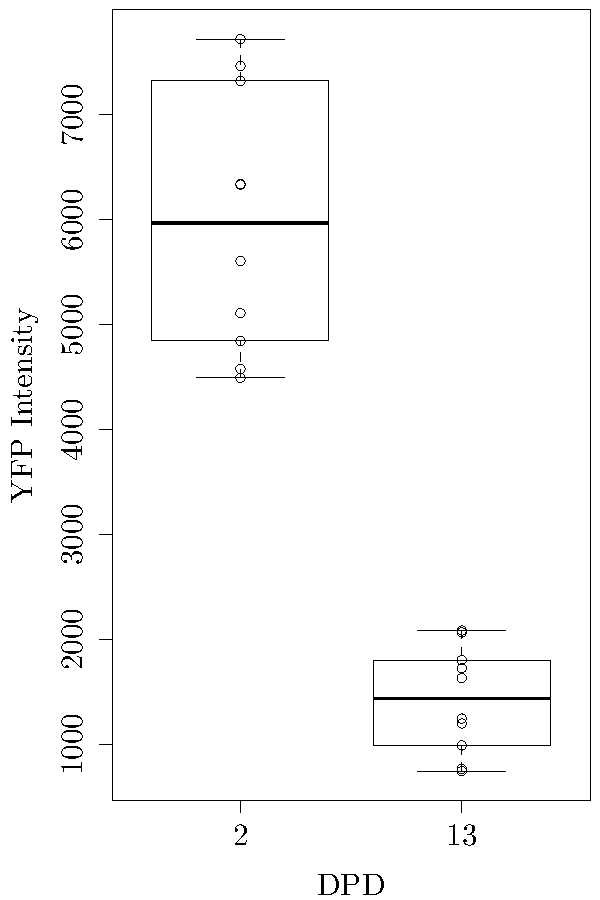
\includegraphics[width=0.38\textwidth]{figures/imprint-off2.pdf}};
      \node[pic] (on)    [right= of off,label={above left:C}]        {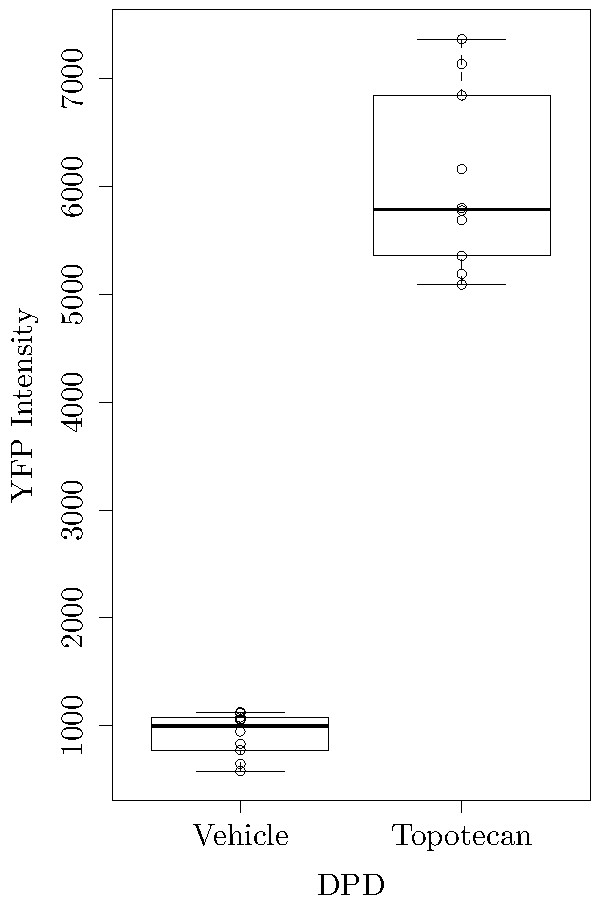
\includegraphics[width=0.38\textwidth]{figures/imprint-on2.pdf}};
      \node[pic] (empty) [above right=0.5mm of off]                  {};
      \node[pic]         [above=0.5mm of empty,label={above left:A}] {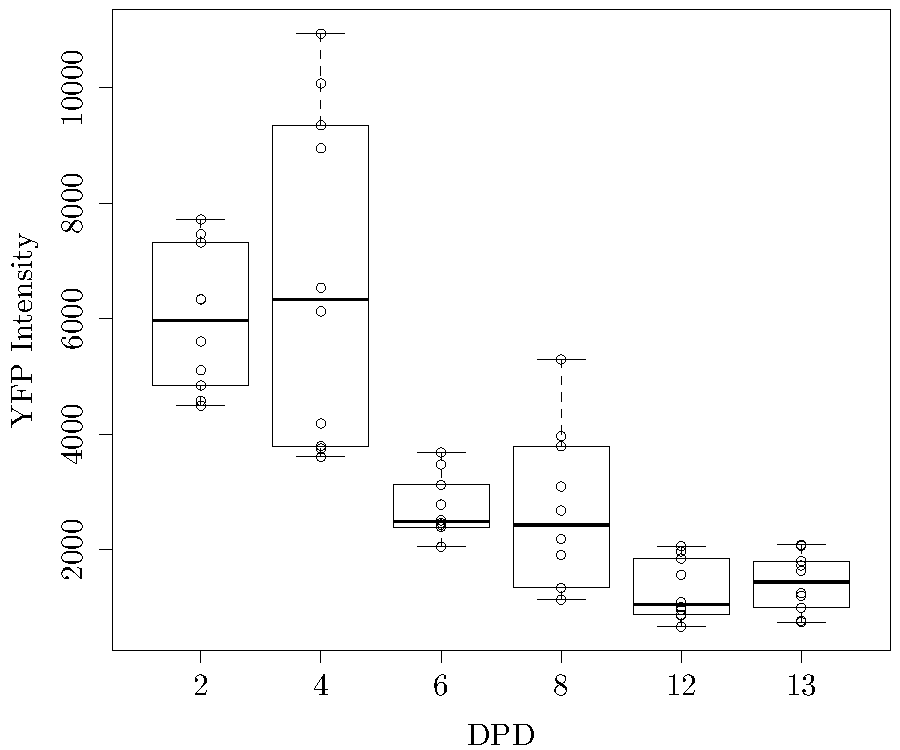
\includegraphics[width=0.75\textwidth]{figures/time-course2.pdf}};
    \end{tikzpicture}
  }
  \caption{Topotecan induces reactivation of paternal \emph{Ube3a} allele in ES cell-derived neurons. \textbf{A)} Boxplots of time course analysis of imprinted neurons (N = 10). \textbf{B)} Boxplots of \emph{Ube3a$^{YFP}$} ES cell-derived neurons at 2 and 13 days post dissociation (DPD) demonstrating the imprinting of paternal \emph{Ube3a}. \textbf{C)} Boxplots of ES cell-derived neurons at 13 DPD with vehicle (water) or Topotecan (300 nM) treatment demonstrating the reactivation of paternal \emph{Ube3a}. N = 15 neurons.}
  \label{Figure 5-1: }
\end{figure}
%%%%%%%%%%%%%%%%%%%%%%%%%%%%%%%%%%%%%%%%%%%%%%%%%%%%%%

\pagebreak

%%%%%%%%%%%%%%%%%%%%%%%%%%%%%%%%%%%%%%%%%%%%%%%%%%%%%%
\begin{longtabu} to \textwidth {X[c]X[c]X[c]X[c]X[c]X[c]X[c]}
  \caption{P-values for time course analysis}\\
  \label{table:5-1}\\
  \toprule
  & \textbf{2 DPD} & \textbf{4 DPD} & \textbf{6 DPD} & \textbf{8 DPD} & \textbf{12 DPD}\\
  \midrule
  \endhead
  \textbf{4 DPD}  & $0.75$               & -                     & -      & -      & -     \\
  \textbf{6 DPD}  & $4.0 \times 10^{-5}$ & $7.3 \times 10^{-7}$  & -      & -      & -     \\
  \textbf{8 DPD}  & $3.5 \times 10^{-5}$ & $6.2 \times 10^{-7}$  & $1.00$ & -      & -     \\
  \textbf{12 DPD} & $2.2 \times 10^{-8}$ & $3.4 \times 10^{-10}$ & $0.24$ & $0.24$ & -     \\
  \textbf{13 DPD} & $4.4 \times 10^{-8}$ & $6.9 \times 10^{-10}$ & $0.28$ & $0.28$ & $1.00$\\
  \bottomrule
\end{longtabu}
%%%%%%%%%%%%%%%%%%%%%%%%%%%%%%%%%%%%%%%%%%%%%%%%%%%%%%

\subsection{Plate effect is not observed for the \textbf{NeuN-Overlap} method}

%%%%%%%%%%%%%%%%%%%%%%%%%%%%%%%%%%%%%%%%%%%%%%%%%%%%%%
\begin{figure}[!h]
  \centering
  \resizebox{\linewidth}{6in}{
    \begin{tikzpicture}[every label/.style={font=\Large\bfseries},pic/.style={inner sep=0pt}]
      \node[pic] {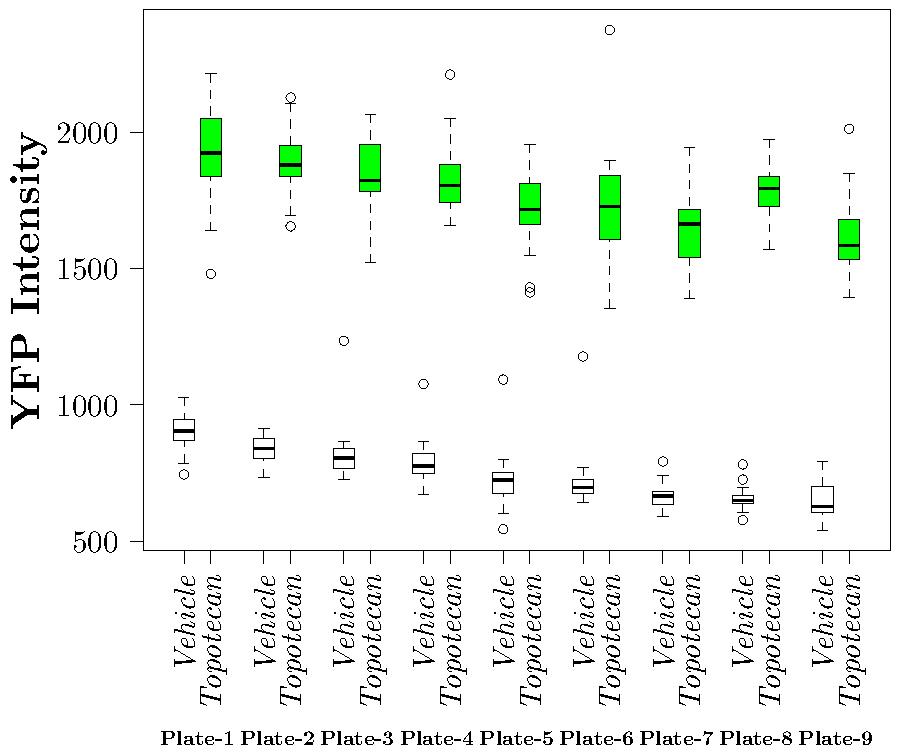
\includegraphics[width=0.90\textwidth]{figures/plate-analysis.pdf}};
    \end{tikzpicture}
  }
  \caption{The decrease in Ube3a$^{YFP}$ intensity as a function of time does not effect separation of Topotecan intensity from Vehicle.}
  \label{Figure 5-2: }
\end{figure}
%%%%%%%%%%%%%%%%%%%%%%%%%%%%%%%%%%%%%%%%%%%%%%%%%%%%%%
To determine if image acquisition time effects the YFP intensity, plate statistics were calculated and plotted in \textbf{Figure \ref{Figure 5-2: }}. Over the course of roughly 12 h, assay stability remains the same with large separation between Vehicle and Topotecan. P-values from the Student's T test were significant for all plates with no correlation over time, \textbf{Table \ref{table:5-2}}. For quality control of assay, the z factor (\textit{Z Factor}) was calculated, \textbf{Table \ref{table:5-2}}; however, since the z factor can be influenced by outliers, the strictly standardized mean difference (SSMD, $\hat{\beta}$) was also calculated, \textbf{Table \ref{table:5-2}}.
\[ Z factor = 1 - \frac{3(\tilde{\sigma}_p + \tilde{\sigma}_n)}{| \tilde{\mu}_p - \tilde{\mu}_n |}, \]
where \( \tilde{\sigma} \) and \( \tilde{\mu} \) are sample standard deviations and sample means, respectively, for positive (\textit{p}) and negative (\textit{n}) controls \cite{Zhang1999,Zhang2011}.
\[ \hat{\beta} = \frac{\tilde{X}_p - \tilde{X}_n}{1.4826\sqrt{\tilde{s}^{2}_p + \tilde{s}^2_n}}, \]
where \( \tilde{X} \) and \( \tilde{s} \) are medians and median absolute deviations in the positive and negative controls, respectively \cite{Zhang2011,Zhang2011b}.

Although assay quality remains the same over time, there is a slight decrease in YFP intensity over time. As a high-throughput assay, plates are often run in large quantities. To determine a theoretical number of plates that can be run at one time, linear regression models were estimated as a function of time for Vehicle YFP intensity (\( R^2 = 0.9645 \)) and Topotecan intensity (\( R^2 = 0.7768 \)). Each plate has roughly 90 min separating them as determined from acquisition log information.
\[ y(Topotecan) = -0.38t + 1911 \ \ \textrm{and} \ \ y(Vehicle) = -0.36t + 879 \]
Set max Vehicle to equal Topotecan to determine when time adversely effects the assay.
\[ 879 = -0.38t + 1911 \]
\[ 879 - 1911 = -0.38t \]
\[ -1032 = -0.38t \]
\[ t = \frac{1032}{0.38}  = 2716 \ \ \textrm{min} \ \ \]
At roughly 90 min image acquisition time, \textbf{NeuN-Overlap} method could ideally run 30 plates assuming antibody decay rate is not exponential. Using more conservative parameters, three times the mean standard deviation of both Topotecan (T) and Vehicle (V), the stability of data acquisition as a function of time is calculated below:
\[ y(T) = -0.38t + 1911 - (3 \times 139.3) \ \ \textrm{and} \ \ y(V) = -0.36t + 879 + (3 \times 67.0) \]
\[ 1080 = -0.38t + 1493 \]
\[ 1080 - 1493 = -0.38t \]
\[ t = \frac{413}{0.38} = 1087 \ \ \textrm{min} \ \ \]
At roughly 90 min image acquisition time, \textbf{NeuN-Overlap} method can conceivably run 12 plates.

%%%%%%%%%%%%%%%%%%%%%%%%%%%%%%%%%%%%%%%%%%%%%%%%%%%%%%
\begin{longtabu} to 5in {X[l]X[c]X[c]X[c]}
  \caption{P-values for \textbf{NeuN-Overlap} plate effect analysis}\\
  \label{table:5-2}\\
  \toprule
  & \textbf{T-test} & \textbf{Z factor} & \textbf{SSMD}\\
  \midrule
  \endhead
  \textbf{Plate-1}  & $1.43 \times 10^{-27}$ & $0.335$ & $5.89$  \\
  \textbf{Plate-2}  & $3.08 \times 10^{-36}$ & $0.526$ & $9.28$  \\
  \textbf{Plate-3}  & $2.68 \times 10^{-31}$ & $0.324$ & $7.54$  \\
  \textbf{Plate-4}  & $8.24 \times 10^{-38}$ & $0.436$ & $8.37$  \\
  \textbf{Plate-5}  & $1.13 \times 10^{-30}$ & $0.311$ & $7.49$  \\
  \textbf{Plate-6}  & $6.37 \times 10^{-21}$ & $0.136$ & $5.87$  \\
  \textbf{Plate-7}  & $3.24 \times 10^{-26}$ & $0.433$ & $6.98$  \\
  \textbf{Plate-8}  & $1.14 \times 10^{-34}$ & $0.629$ & $13.65$ \\
  \textbf{Plate-9}  & $1.63 \times 10^{-28}$ & $0.389$ & $7.34$  \\
  \bottomrule
\end{longtabu}
%%%%%%%%%%%%%%%%%%%%%%%%%%%%%%%%%%%%%%%%%%%%%%%%%%%%%%

\subsection{Well position effects Ube3a$^{YFP}$ intensity}

To determine if well position effected YFP intensity measured, wells with vehicle from column 1 were compared with vehicle from column 24, and Topotecan wells from column 2 were compared with Topotecan wells from column 23. The p-values from the two-tailed Student's T-test are shown in \textbf{Table \ref{table:5-3}}. Only two plates for Vehicle show well position effects, while Topotecan wells have nearly half showing significant differences between positions within the plate. 

\pagebreak
%%%%%%%%%%%%%%%%%%%%%%%%%%%%%%%%%%%%%%%%%%%%%%%%%%%%%%
\begin{longtabu} to 4in {X[l]X[c]X[c]}
  \caption{P-values (T-test) for \textbf{NeuN-Overlap} well effect analysis}\\
  \label{table:5-3}\\
  \toprule
  & \textbf{Vehicle} & \textbf{Topotecan}\\
  \midrule
  \endhead
  \textbf{Plate-1}  & $0.005$ & $0.170$ \\
  \textbf{Plate-2}  & $0.001$ & $0.017$ \\
  \textbf{Plate-3}  & $0.249$ & $0.021$ \\
  \textbf{Plate-4}  & $0.117$ & $0.507$ \\
  \textbf{Plate-5}  & $0.234$ & $ <0.001$ \\
  \textbf{Plate-6}  & $0.218$ & $0.228$ \\
  \textbf{Plate-7}  & $0.114$ & $0.003$ \\
  \textbf{Plate-8}  & $0.285$ & $0.382$ \\
  \textbf{Plate-9}  & $0.500$ & $0.194$ \\
  \bottomrule
\end{longtabu}
%%%%%%%%%%%%%%%%%%%%%%%%%%%%%%%%%%%%%%%%%%%%%%%%%%%%%%

\section{Discussion}

In this chapter, the high-throughput screening method developed in \textbf{Chapter 4} is validated via proof-of-concept screening for Angelman syndrome. Embryonic stem cells were generated from reporter mice \textit{Ube3a$^{+/YFP}$} \cite{Dindot2008} and expanded. The expansion of these ES cells provides a large pool of available ES cells at the same time point for further differentiation. The neurons derived from these ES cells were significantly more than those that can be collected from primary cultures with on average $600 \times 10^6$ from 6 initial neuronal induction plates. For neurons obtained from embryonic mice, the generation of animals presents a major bottleneck for high-throughput screening. Even with recent advances in neuron mini-cultures, 1 million cells can only plate little more than four 384-well plates \cite{Niedringhaus2015}. To compare, mini-cultures would still require more than 200 embryos with excellent culturing techniques to generate similar numbers.

As research has shown that paternal \textit{Ube3a} is imprinting during development, the time point of imprinting of paternal \textit{Ube3a} in culture was determined for the HTS assay. We determined that within six days Ube3a$^{YFP}$ significantly decreased. For the HTS assay, drugs were added 7 DPD for convenience of HTS facility. Nine 384-well optical-bottom plates were run with Vehicle, columns 1 \& 24, and Topotecan, columns 2 \& 23, added to the plate using a 300 drugs/small molecule compounds drug loading model. At roughly 30 min/antibody, the total plate image acquisition time was approximately 90 min/plate, which is longer than most HTS that commonly only image with a single antibody. As such, there was some concern that antibody intensity would significantly decrease overtime; however, using the NeuN-Overlap, which is specific to mature neurons, there was no significant decrease observed. Even so, it is this author's recommendation that only 12 plates be run in one sitting assuming that acquisition time is approximately 90 min.

All plates showed significant difference between Vehicle and Topotecan controls, \textbf{Table \ref{table:5-2}}; however, only two plates had a z factor of $\geq$ 0.5, which indicates an \textit{Excellent} assay \cite{Zhang1999}. This may be due to the outliers observed in \textbf{Figure \ref{Figure 5-2: }} as the z factor calculation is not robust to outliers \cite{Sui2007}. As an alternative, the strictly standardized mean difference method specific to outliers robustness was also calculated per plate with an average $\hat{\beta}$ of approximately 8.04, where $\hat{\beta} > 7.0$ is an \textit{Excellent} assay for HTS small molecule assays \cite{Zhang2011}. Altogether using the outliers robust SSMD method, this HTS assay scores an \textit{Excellent} for quality control.

Finally, this work is directly applicable for preforming a high-throughput screen for Angelman syndrome. Currently, the only drug known to reactivate the paternal \textit{Ube3a} allele is Topotecan. This drug, however, is extremely toxic and currently approved as a chemotherapeutic. Therefore, an alternative therapeutic drug is still needed. Furthermore with this ES cell-derived neuronal culture HTS assay, it will be possible to conduct an RNA interference screen for pathway analysis of the imprint of \textit{Ube3a}. With such a screen, additional targets for therapeutic intervention for Angelman syndrome can possibly be determined. In summary, this data shows that ES-N model can dramatically increase the scale of screening studies for neurological disorders.
